\PassOptionsToPackage{unicode=true}{hyperref} % options for packages loaded elsewhere
\PassOptionsToPackage{hyphens}{url}
%
\documentclass[]{article}
\usepackage{lmodern}
\usepackage{amssymb,amsmath}
\usepackage{ifxetex,ifluatex}
\usepackage{fixltx2e} % provides \textsubscript
\ifnum 0\ifxetex 1\fi\ifluatex 1\fi=0 % if pdftex
  \usepackage[T1]{fontenc}
  \usepackage[utf8]{inputenc}
  \usepackage{textcomp} % provides euro and other symbols
\else % if luatex or xelatex
  \usepackage{unicode-math}
  \defaultfontfeatures{Ligatures=TeX,Scale=MatchLowercase}
\fi
% use upquote if available, for straight quotes in verbatim environments
\IfFileExists{upquote.sty}{\usepackage{upquote}}{}
% use microtype if available
\IfFileExists{microtype.sty}{%
\usepackage[]{microtype}
\UseMicrotypeSet[protrusion]{basicmath} % disable protrusion for tt fonts
}{}
\IfFileExists{parskip.sty}{%
\usepackage{parskip}
}{% else
\setlength{\parindent}{0pt}
\setlength{\parskip}{6pt plus 2pt minus 1pt}
}
\usepackage{hyperref}
\hypersetup{
            pdftitle={Algoritma Academy: Practical Statistics},
            pdfauthor={Samuel Chan},
            pdfborder={0 0 0},
            breaklinks=true}
\urlstyle{same}  % don't use monospace font for urls
\usepackage[margin=1in]{geometry}
\usepackage{color}
\usepackage{fancyvrb}
\newcommand{\VerbBar}{|}
\newcommand{\VERB}{\Verb[commandchars=\\\{\}]}
\DefineVerbatimEnvironment{Highlighting}{Verbatim}{commandchars=\\\{\}}
% Add ',fontsize=\small' for more characters per line
\usepackage{framed}
\definecolor{shadecolor}{RGB}{248,248,248}
\newenvironment{Shaded}{\begin{snugshade}}{\end{snugshade}}
\newcommand{\AlertTok}[1]{\textcolor[rgb]{0.94,0.16,0.16}{#1}}
\newcommand{\AnnotationTok}[1]{\textcolor[rgb]{0.56,0.35,0.01}{\textbf{\textit{#1}}}}
\newcommand{\AttributeTok}[1]{\textcolor[rgb]{0.77,0.63,0.00}{#1}}
\newcommand{\BaseNTok}[1]{\textcolor[rgb]{0.00,0.00,0.81}{#1}}
\newcommand{\BuiltInTok}[1]{#1}
\newcommand{\CharTok}[1]{\textcolor[rgb]{0.31,0.60,0.02}{#1}}
\newcommand{\CommentTok}[1]{\textcolor[rgb]{0.56,0.35,0.01}{\textit{#1}}}
\newcommand{\CommentVarTok}[1]{\textcolor[rgb]{0.56,0.35,0.01}{\textbf{\textit{#1}}}}
\newcommand{\ConstantTok}[1]{\textcolor[rgb]{0.00,0.00,0.00}{#1}}
\newcommand{\ControlFlowTok}[1]{\textcolor[rgb]{0.13,0.29,0.53}{\textbf{#1}}}
\newcommand{\DataTypeTok}[1]{\textcolor[rgb]{0.13,0.29,0.53}{#1}}
\newcommand{\DecValTok}[1]{\textcolor[rgb]{0.00,0.00,0.81}{#1}}
\newcommand{\DocumentationTok}[1]{\textcolor[rgb]{0.56,0.35,0.01}{\textbf{\textit{#1}}}}
\newcommand{\ErrorTok}[1]{\textcolor[rgb]{0.64,0.00,0.00}{\textbf{#1}}}
\newcommand{\ExtensionTok}[1]{#1}
\newcommand{\FloatTok}[1]{\textcolor[rgb]{0.00,0.00,0.81}{#1}}
\newcommand{\FunctionTok}[1]{\textcolor[rgb]{0.00,0.00,0.00}{#1}}
\newcommand{\ImportTok}[1]{#1}
\newcommand{\InformationTok}[1]{\textcolor[rgb]{0.56,0.35,0.01}{\textbf{\textit{#1}}}}
\newcommand{\KeywordTok}[1]{\textcolor[rgb]{0.13,0.29,0.53}{\textbf{#1}}}
\newcommand{\NormalTok}[1]{#1}
\newcommand{\OperatorTok}[1]{\textcolor[rgb]{0.81,0.36,0.00}{\textbf{#1}}}
\newcommand{\OtherTok}[1]{\textcolor[rgb]{0.56,0.35,0.01}{#1}}
\newcommand{\PreprocessorTok}[1]{\textcolor[rgb]{0.56,0.35,0.01}{\textit{#1}}}
\newcommand{\RegionMarkerTok}[1]{#1}
\newcommand{\SpecialCharTok}[1]{\textcolor[rgb]{0.00,0.00,0.00}{#1}}
\newcommand{\SpecialStringTok}[1]{\textcolor[rgb]{0.31,0.60,0.02}{#1}}
\newcommand{\StringTok}[1]{\textcolor[rgb]{0.31,0.60,0.02}{#1}}
\newcommand{\VariableTok}[1]{\textcolor[rgb]{0.00,0.00,0.00}{#1}}
\newcommand{\VerbatimStringTok}[1]{\textcolor[rgb]{0.31,0.60,0.02}{#1}}
\newcommand{\WarningTok}[1]{\textcolor[rgb]{0.56,0.35,0.01}{\textbf{\textit{#1}}}}
\usepackage{longtable,booktabs}
% Fix footnotes in tables (requires footnote package)
\IfFileExists{footnote.sty}{\usepackage{footnote}\makesavenoteenv{longtable}}{}
\usepackage{graphicx,grffile}
\makeatletter
\def\maxwidth{\ifdim\Gin@nat@width>\linewidth\linewidth\else\Gin@nat@width\fi}
\def\maxheight{\ifdim\Gin@nat@height>\textheight\textheight\else\Gin@nat@height\fi}
\makeatother
% Scale images if necessary, so that they will not overflow the page
% margins by default, and it is still possible to overwrite the defaults
% using explicit options in \includegraphics[width, height, ...]{}
\setkeys{Gin}{width=\maxwidth,height=\maxheight,keepaspectratio}
\setlength{\emergencystretch}{3em}  % prevent overfull lines
\providecommand{\tightlist}{%
  \setlength{\itemsep}{0pt}\setlength{\parskip}{0pt}}
\setcounter{secnumdepth}{0}
% Redefines (sub)paragraphs to behave more like sections
\ifx\paragraph\undefined\else
\let\oldparagraph\paragraph
\renewcommand{\paragraph}[1]{\oldparagraph{#1}\mbox{}}
\fi
\ifx\subparagraph\undefined\else
\let\oldsubparagraph\subparagraph
\renewcommand{\subparagraph}[1]{\oldsubparagraph{#1}\mbox{}}
\fi

% set default figure placement to htbp
\makeatletter
\def\fps@figure{htbp}
\makeatother


\title{Algoritma Academy: Practical Statistics}
\author{Samuel Chan}
\date{21 August, 2020}

\begin{document}
\maketitle

\hypertarget{background}{%
\section{Background}\label{background}}

\hypertarget{algoritma}{%
\subsection{Algoritma}\label{algoritma}}

The following coursebook is produced by the team at
\href{https://algorit.ma}{Algoritma} for its Data Science Academy
workshops. The coursebook is intended for a restricted audience only,
i.e.~the individuals and organizations having received this coursebook
directly from the training organization. It may not be reproduced,
distributed, translated or adapted in any form outside these individuals
and organizations without permission.

Algoritma is a data science education center with bootcamp programs
offered in:

\begin{itemize}
\tightlist
\item
  Bahasa Indonesia (Jakarta campus)\\
\item
  English (Singapore campus)
\end{itemize}

\hypertarget{lifelong-learning-benefits}{%
\subsubsection{Lifelong Learning
Benefits}\label{lifelong-learning-benefits}}

If you're an active student or an alumni member, you also qualify for
all our future workshops, 100\% free of charge as part of your
\textbf{lifelong learning benefits}. It is a new initiative to help you
gain mastery and advance your knowledge in the field of data
visualization, machine learning, computer vision, natural language
processing (NLP) and other sub-fields of data science. All workshops
conducted by us (from 1-day to 5-day series) are available to you
free-of-charge, and the benefits \textbf{never expire}.

\hypertarget{second-edition}{%
\subsubsection{Second Edition}\label{second-edition}}

This coursebook is initially written in 2017.

This is the second edition, written in late August 2020. Some of the
code has been refactored to work with the latest major version of R,
version 4.0. I would like to thank the incredible instructor team at
Algoritma for their thorough input and assistance in the authoring and
reviewing process.

\hypertarget{libraries-and-setup}{%
\subsection{Libraries and Setup}\label{libraries-and-setup}}

We'll set-up caching for this notebook given how computationally
expensive some of the code we will write can get.

\begin{Shaded}
\begin{Highlighting}[]
\KeywordTok{options}\NormalTok{(}\DataTypeTok{scipen =} \DecValTok{9999}\NormalTok{)}
\KeywordTok{rm}\NormalTok{(}\DataTypeTok{list=}\KeywordTok{ls}\NormalTok{())}
\end{Highlighting}
\end{Shaded}

You will need to use \texttt{install.packages()} to install any packages
that are not already downloaded onto your machine. You then load the
package into your workspace using the \texttt{library()} function:

\begin{Shaded}
\begin{Highlighting}[]
\KeywordTok{library}\NormalTok{(skimr)}
\end{Highlighting}
\end{Shaded}

\hypertarget{training-objectives}{%
\subsection{Training Objectives}\label{training-objectives}}

The primary objective of this course is to pave the statistical
foundation for more advanced machine learning theories later on in the
specialization. The syllabus covers:

\begin{itemize}
\item
  \textbf{Descriptive Statistics}
\item
  5 Number Summary
\item
  Statistical Plots for Descriptive Statistics\\
\item
  Working with Quantiles\\
\item
  Central Tendency and Variability
\item
  z-Score and Central Limit Theorem
\item
  \textbf{Inferential Statistics}\\
\item
  Probability Mass Function
\item
  Probability Density Function
\item
  Confidence Intervals\\
\item
  Hypothesis Test
\item
  p-Value Interpretation
\end{itemize}

By the end of the workshop, Academy students are required to complete
one the following Learn-By-Building project:

\textbf{Descriptive Statistics}\\
Use a combination of statistical tools and plots to explain what you've
learned from the data. Include at least 3 statistical plots, as well as
a summary paragraph to describe any findings or points of interest at
this stage.

The learn-by-building project in this course is not graded.

\hypertarget{descriptive-statistics}{%
\section{Descriptive Statistics}\label{descriptive-statistics}}

Statisticians and data scientists use descriptive statistics to
summarize and describe a large number of measurements. Many times, this
task is accompanied with graphs and plots that help describe the
numerical summary of data. When data science is applied in the business
context, an example of descriptive statistic is the average number of
transactions per month. Another example is the percentage of e-commerce
transactions with a voucher code applied. The simple rule is that
descriptive statistics \textbf{do not involve generalizing beyond the
data we have obtained, and are merely descriptive of what we have at
hand}. The branch of statistics that deal with drawing inferences about
the larger population is called inferential statistics.

Let's start by reading in the \texttt{retail} dataset:

\begin{Shaded}
\begin{Highlighting}[]
\NormalTok{retail <-}\StringTok{ }\KeywordTok{read.csv}\NormalTok{(}\StringTok{"data_input/workshop.csv"}\NormalTok{)}
\end{Highlighting}
\end{Shaded}

Notice that because we did not pass the \texttt{stringsAsFactors=F}
parameter, the function's default behavior is to convert any character
variables into factor variables. In the last workshop we learned how to
use \texttt{as.Date} and \texttt{as.character} to transform variables
into the desired type but here let's see how we can combine these two
``converter'' functions with \texttt{lapply} to make our code more
concise:

\begin{Shaded}
\begin{Highlighting}[]
\NormalTok{retail[,}\DecValTok{1}\OperatorTok{:}\DecValTok{2}\NormalTok{] <-}\StringTok{ }\KeywordTok{lapply}\NormalTok{(retail[,}\DecValTok{1}\OperatorTok{:}\DecValTok{2}\NormalTok{], as.Date)}
\NormalTok{retail[,}\KeywordTok{c}\NormalTok{(}\StringTok{"Customer.ID"}\NormalTok{, }\StringTok{"Product.Name"}\NormalTok{)] <-}\StringTok{ }\KeywordTok{lapply}\NormalTok{(retail[, }\KeywordTok{c}\NormalTok{(}\StringTok{"Customer.ID"}\NormalTok{, }\StringTok{"Product.Name"}\NormalTok{)], as.character)}
\end{Highlighting}
\end{Shaded}

In the first line of code, \texttt{lapply} takes \texttt{as.Date} as a
function and apply that function over the first two variables:
\texttt{Order.Date} and \texttt{Ship.Date}. Notice that with
\texttt{lapply} instead of writing 4 or 5 converter functions, each time
substituting the variable names, we could just do it in one go!

In describing data, we are typically concerned with the task of
quantifying and comparing \textbf{central tendency},
\textbf{variability}, and the \textbf{shape} of our data.

\hypertarget{measures-of-central-tendency}{%
\subsection{Measures of Central
Tendency}\label{measures-of-central-tendency}}

Often times in the exploratory data analysis phase, we want to get a
sense of what the \emph{most representative score} of a particular
measurement is. We often simplify this idea by referring to it as the
``average'', but there are in fact, three measures of central tendency
that you need to have in your statistical toolset.

The most popular measure of central tendency is the \emph{mean}, which
is sometimes represented as \(\bar{x}\) when computed on a \emph{sample}
and represented as \(\mu\) when computed on a population. Mean is really
the sum of all your measurements, divided by the number of measurements,
and works best on data that has an even distribution or a normal
distribution (don't worry if the idea of a normal distribution isn't
clear - we'll get to that in a while!). In R, the \texttt{mean} function
will return the mean:

\begin{Shaded}
\begin{Highlighting}[]
\KeywordTok{sum}\NormalTok{(retail}\OperatorTok{$}\NormalTok{Profit)}\OperatorTok{/}\KeywordTok{length}\NormalTok{(retail}\OperatorTok{$}\NormalTok{Profit)}
\end{Highlighting}
\end{Shaded}

\begin{verbatim}
## [1] 28.6569
\end{verbatim}

\begin{Shaded}
\begin{Highlighting}[]
\KeywordTok{mean}\NormalTok{(retail}\OperatorTok{$}\NormalTok{Profit)}
\end{Highlighting}
\end{Shaded}

\begin{verbatim}
## [1] 28.6569
\end{verbatim}

The median is the point of value that cuts the distribution into two
equal halves such that 50\% of the observations are below it. To find
this value, we would order the observations and find the middle value
that separates the distribution into two equal halves.

\begin{Shaded}
\begin{Highlighting}[]
\NormalTok{shipment.kg <-}\StringTok{ }\KeywordTok{c}\NormalTok{(}\DecValTok{5}\NormalTok{,}\DecValTok{10}\NormalTok{,}\DecValTok{2}\NormalTok{,}\DecValTok{3}\NormalTok{,}\DecValTok{7}\NormalTok{)}
\CommentTok{# when we order it, we see the middle value being 5}
\NormalTok{shipment.kg[}\KeywordTok{order}\NormalTok{(shipment.kg)]}
\end{Highlighting}
\end{Shaded}

\begin{verbatim}
## [1]  2  3  5  7 10
\end{verbatim}

\begin{Shaded}
\begin{Highlighting}[]
\CommentTok{# using median() yield the same result}
\KeywordTok{median}\NormalTok{(shipment.kg)}
\end{Highlighting}
\end{Shaded}

\begin{verbatim}
## [1] 5
\end{verbatim}

For data with odd number of observations, the median is the middle value
but for data with an even number of observations we would instead use
the average of the two middle scores:

\begin{Shaded}
\begin{Highlighting}[]
\NormalTok{shipment.cost <-}\StringTok{ }\KeywordTok{c}\NormalTok{(}\DecValTok{5}\NormalTok{,}\DecValTok{10}\NormalTok{,}\DecValTok{2}\NormalTok{,}\DecValTok{6}\NormalTok{,}\DecValTok{8}\NormalTok{,}\DecValTok{8}\NormalTok{)}
\CommentTok{# when we order it, we see the middle value being 7}
\NormalTok{shipment.cost[}\KeywordTok{order}\NormalTok{(shipment.cost)]}
\end{Highlighting}
\end{Shaded}

\begin{verbatim}
## [1]  2  5  6  8  8 10
\end{verbatim}

\begin{Shaded}
\begin{Highlighting}[]
\CommentTok{# using median() yield the same result}
\KeywordTok{median}\NormalTok{(shipment.cost)}
\end{Highlighting}
\end{Shaded}

\begin{verbatim}
## [1] 7
\end{verbatim}

We need to be cautious when applying the \texttt{mean} on data with a
skewed distribution because the mean may not be the best candidate for a
\textbf{most representative score} compared to other measures of central
tendency. For example, a company surveys its employees household income
and posted the following monthly household income (IDR, in Mil):

\begin{Shaded}
\begin{Highlighting}[]
\NormalTok{salary <-}\StringTok{ }\KeywordTok{c}\NormalTok{(}\FloatTok{7.8}\NormalTok{, }\FloatTok{7.5}\NormalTok{, }\DecValTok{6}\NormalTok{, }\FloatTok{7.5}\NormalTok{, }\FloatTok{4.5}\NormalTok{, }\DecValTok{105}\NormalTok{, }\DecValTok{45}\NormalTok{, }\FloatTok{7.5}\NormalTok{, }\FloatTok{5.5}\NormalTok{, }\DecValTok{4}\NormalTok{)}
\KeywordTok{mean}\NormalTok{(salary)}
\end{Highlighting}
\end{Shaded}

\begin{verbatim}
## [1] 20.03
\end{verbatim}

\begin{Shaded}
\begin{Highlighting}[]
\KeywordTok{median}\NormalTok{(salary)}
\end{Highlighting}
\end{Shaded}

\begin{verbatim}
## [1] 7.5
\end{verbatim}

While the median puts that figure at about 7.25, the mean is about 2.67
times higher and is not truly representative of the actual household
income. While most of the employees have a combined household earning of
less than 8 mil, the mean value of our household income would have
believe that the average household income of our employees is in fact
more than 20 mil IDR.

The median in this case is a better measure of centrality because it is
not sensitive to the outlier data.

If we are in fact, \emph{required} to compute the mean on data with
skewed distribution, another technique to reduce the influence of
outlier data is to use a slight variation of the mean, called the
Trimmed Mean. The trimmed mean removes a small designated percentage of
the largest and smallest values before computing the mean. A trimmed
mean that computes the middle 95\% of the distribution can be performed
in R fairly easily:

\begin{Shaded}
\begin{Highlighting}[]
\CommentTok{# 5% of observations to be trimmed}
\KeywordTok{mean}\NormalTok{(retail}\OperatorTok{$}\NormalTok{Profit, }\DataTypeTok{trim =} \FloatTok{0.05}\NormalTok{)}
\end{Highlighting}
\end{Shaded}

\begin{verbatim}
## [1] 19.16937
\end{verbatim}

When there are discreet values fora variable, the statisyical mode
refers to the value that occurs most frequently. This statistic is
rarely used in practice. Say we are surveying the number of times a
customer place a booking in our travel booking app over the period of a
year and collected the following sample:

\begin{Shaded}
\begin{Highlighting}[]
\NormalTok{numberoftravels <-}\StringTok{ }\KeywordTok{c}\NormalTok{(}\DecValTok{2}\NormalTok{,}\DecValTok{2}\NormalTok{,}\DecValTok{3}\NormalTok{,}\DecValTok{1}\NormalTok{,}\DecValTok{0}\NormalTok{,}\DecValTok{4}\NormalTok{,}\DecValTok{2}\NormalTok{,}\DecValTok{5}\NormalTok{,}\DecValTok{1}\NormalTok{,}\DecValTok{2}\NormalTok{,}\DecValTok{4}\NormalTok{)}

\NormalTok{most <-}\StringTok{ }\ControlFlowTok{function}\NormalTok{(x)\{}
  \KeywordTok{as.integer}\NormalTok{(}\KeywordTok{names}\NormalTok{(}\KeywordTok{sort}\NormalTok{(}\OperatorTok{-}\KeywordTok{table}\NormalTok{(x)))[}\DecValTok{1}\NormalTok{])}
\NormalTok{\}}

\KeywordTok{most}\NormalTok{(numberoftravels)}
\end{Highlighting}
\end{Shaded}

\begin{verbatim}
## [1] 2
\end{verbatim}

Because R do not have a built-in way of computing the mode, we wrote the
code above to tabulate our data (using \texttt{table}), multiply the
calculation by -1 (and hence giving it the effect of sorting our data in
descending order) and then pick the first value.

\hypertarget{measures-of-spread}{%
\subsection{Measures of Spread}\label{measures-of-spread}}

Measures of spread measures the extent to which \textbf{value in a
distribution differ from each other}. In practice, it is far easier to
compute the distance between the values to their mean and when we square
each one of these distances and add them all up the average\footnote{While
  I use the word \emph{average}, the sum of squared difference is in
  fact divided by \(n-1\) instead of \(n\) when we're estimating the
  standard deviation (or variance) of the population from the equivalent
  sample statistic. This is because the observed values fall on average
  closer to the sample mean than the population mean, the standard
  deviation which is calculated using deviations from the sample mean
  underestimates the desired standard deviation of the population. Using
  \(n-1\) instead of \(n\) as the divisor corrects for that
  ``underestimation'' by making the result a little bigger.} of that
result is known as \textbf{variance}. Taking the square root of the
variance will result in the \textbf{standard deviation}. Just like the
mean, standard deviation is the ``expected value'' of how far the scores
deviate from the mean.

\begin{Shaded}
\begin{Highlighting}[]
\KeywordTok{sum}\NormalTok{((numberoftravels }\OperatorTok{-}\StringTok{ }\KeywordTok{mean}\NormalTok{(numberoftravels))}\OperatorTok{^}\DecValTok{2}\NormalTok{)}\OperatorTok{/}\NormalTok{(}\KeywordTok{length}\NormalTok{(numberoftravels)}\OperatorTok{-}\DecValTok{1}\NormalTok{)}
\end{Highlighting}
\end{Shaded}

\begin{verbatim}
## [1] 2.254545
\end{verbatim}

\begin{Shaded}
\begin{Highlighting}[]
\KeywordTok{var}\NormalTok{(numberoftravels)}
\end{Highlighting}
\end{Shaded}

\begin{verbatim}
## [1] 2.254545
\end{verbatim}

And taking the square root of variance yields the standard deviation:

\begin{Shaded}
\begin{Highlighting}[]
\KeywordTok{sqrt}\NormalTok{(}\KeywordTok{var}\NormalTok{(numberoftravels))}
\end{Highlighting}
\end{Shaded}

\begin{verbatim}
## [1] 1.501514
\end{verbatim}

\begin{Shaded}
\begin{Highlighting}[]
\KeywordTok{sd}\NormalTok{(numberoftravels)}
\end{Highlighting}
\end{Shaded}

\begin{verbatim}
## [1] 1.501514
\end{verbatim}

Variance and standard deviation are always positive when the values are
not identical. When there's no variability, the variance is 0. Because
variance and standard deviation are sensitive to every value, they may
not be the most ``representative'' measurement for skewed data.

Other measurements of the spread are the \textbf{range} and the
\textbf{interquartile range}. The range is the distance from our
smallest measurement to the largest one:

\begin{Shaded}
\begin{Highlighting}[]
\KeywordTok{max}\NormalTok{(numberoftravels) }\OperatorTok{-}\StringTok{ }\KeywordTok{min}\NormalTok{(numberoftravels)}
\end{Highlighting}
\end{Shaded}

\begin{verbatim}
## [1] 5
\end{verbatim}

\begin{Shaded}
\begin{Highlighting}[]
\KeywordTok{diff}\NormalTok{(}\KeywordTok{range}\NormalTok{(numberoftravels))}
\end{Highlighting}
\end{Shaded}

\begin{verbatim}
## [1] 5
\end{verbatim}

The interquartile range is the range computed for the middle 50\% of the
distribution:

\begin{Shaded}
\begin{Highlighting}[]
\KeywordTok{IQR}\NormalTok{(numberoftravels)}
\end{Highlighting}
\end{Shaded}

\begin{verbatim}
## [1] 2
\end{verbatim}

\begin{Shaded}
\begin{Highlighting}[]
\KeywordTok{as.numeric}\NormalTok{(}\KeywordTok{quantile}\NormalTok{(numberoftravels, }\FloatTok{0.75}\NormalTok{) }\OperatorTok{-}\StringTok{ }\KeywordTok{quantile}\NormalTok{(numberoftravels, }\FloatTok{0.25}\NormalTok{))}
\end{Highlighting}
\end{Shaded}

\begin{verbatim}
## [1] 2
\end{verbatim}

While we can use \texttt{quantile()} to obtain the 3rd and 1st quartile
individually, these two figures are also presented together with the 0th
(the \texttt{min()}), 50th (the \texttt{median()}), and the 100th (the
\texttt{max()}) quartiles: together they are called the five-number
summary.

When we call \texttt{fivenum()}, we get this summary that we can use as
a measure of variation for even potentially skewed data:

\begin{Shaded}
\begin{Highlighting}[]
\KeywordTok{fivenum}\NormalTok{(retail}\OperatorTok{$}\NormalTok{Profit)}
\end{Highlighting}
\end{Shaded}

\begin{verbatim}
## [1] -6599.9780     1.7280     8.6665    29.3640  8399.9760
\end{verbatim}

From the above, observe that the absolute lowest profit (the
\texttt{min}) approximates 6,600 and the highest profit approximates
8,400 (the \texttt{max}); Observe also that 25\% of our transactions
make a profit of less than 1.728. Half of the transactions (the middle
50\% of the value) make a profit between 1.728 and 29.364 - recall that
this range is called the \emph{interquartile range} (IQR). When we use
\texttt{summary()} on continuous data, we'll get the five number summary
and the mean in return:

\begin{Shaded}
\begin{Highlighting}[]
\KeywordTok{summary}\NormalTok{(retail}\OperatorTok{$}\NormalTok{Profit)}
\end{Highlighting}
\end{Shaded}

\begin{verbatim}
##      Min.   1st Qu.    Median      Mean   3rd Qu.      Max. 
## -6599.978     1.729     8.666    28.657    29.364  8399.976
\end{verbatim}

A related concept to standard deviation, that is quite foundational to
inferential statistics when we come to that later, is the standard error
of the mean.

Standard error of the mean is a measure that estimates how close a
calculated mean (sample) is likely to be to the true mean of that
population; It is calculated by dividing the standard deviation of the
sample data by the square root of the number of observations:

\begin{Shaded}
\begin{Highlighting}[]
\KeywordTok{library}\NormalTok{(psych)}
\KeywordTok{sd}\NormalTok{(numberoftravels)}\OperatorTok{/}\KeywordTok{sqrt}\NormalTok{(}\KeywordTok{length}\NormalTok{(numberoftravels))}
\end{Highlighting}
\end{Shaded}

\begin{verbatim}
## [1] 0.4527236
\end{verbatim}

\begin{Shaded}
\begin{Highlighting}[]
\KeywordTok{describe}\NormalTok{(numberoftravels)}\OperatorTok{$}\NormalTok{se}
\end{Highlighting}
\end{Shaded}

\begin{verbatim}
## [1] 0.4527236
\end{verbatim}

On a normal distribution (we'll get to this in a moment), 67\% of the
time the true population mean will lie within the range of +- 1 SE. In
other words, if we can establish a normal distribution, we can theorize
about the true value of the population mean with a range. Because of the
formula:\\
\(SE = \frac{\sigma}{\sqrt{n}}\)

The larger our sample size \emph{n} gets, the smaller SE will be: and
hence we are less uncertain about our estimation of the true population
mean.

\textbf{Quiz 1: Which financial assets has more votality in their annual
price?}

\begin{Shaded}
\begin{Highlighting}[]
\NormalTok{price.coins <-}\StringTok{ }\KeywordTok{c}\NormalTok{(}\FloatTok{1.4}\NormalTok{, }\FloatTok{0.4}\NormalTok{, }\FloatTok{0.8}\NormalTok{, }\FloatTok{1.1}\NormalTok{, }\FloatTok{1.8}\NormalTok{, }\FloatTok{2.2}\NormalTok{, }\FloatTok{2.3}\NormalTok{, }\FloatTok{1.2}\NormalTok{)}
\NormalTok{price.oil <-}\StringTok{ }\KeywordTok{c}\NormalTok{(}\FloatTok{1.6}\NormalTok{, }\FloatTok{1.2}\NormalTok{, }\FloatTok{1.9}\NormalTok{, }\FloatTok{0.8}\NormalTok{, }\FloatTok{0.6}\NormalTok{, }\FloatTok{1.5}\NormalTok{, }\FloatTok{2.1}\NormalTok{, }\FloatTok{1.5}\NormalTok{)}
\end{Highlighting}
\end{Shaded}

The primary measure of votality used by stock traders and financial
analysts is standard deviation, and recall that this metric reflects the
average amount of an item's price over a period of time. While the price
for our fictional ``oil'' asset and ``coins'' asset averaged out to be
USD 1.4 over time, which of these two present a higher votality than the
other?

\hypertarget{covariance-and-correlation}{%
\subsection{Covariance and
Correlation}\label{covariance-and-correlation}}

When we have two samples, X and Y, of the same size, then the covariance
is an estimate of how \textbf{variation in X is related to the variation
in Y}. Covariance measures how two variables \emph{covary} and is
represented as:\\
\(Cov(X, Y) = \frac{1}{n-1}\sum\limits^n_{i=1}(X_i - \mu_X)(Y_i - \mu_Y)\)

\begin{Shaded}
\begin{Highlighting}[]
\KeywordTok{sum}\NormalTok{((price.coins }\OperatorTok{-}\StringTok{ }\KeywordTok{mean}\NormalTok{(price.coins))}\OperatorTok{*}\NormalTok{(price.oil }\OperatorTok{-}\StringTok{ }\KeywordTok{mean}\NormalTok{(price.oil)))}\OperatorTok{/}\NormalTok{(}\KeywordTok{length}\NormalTok{(price.coins)}\OperatorTok{-}\DecValTok{1}\NormalTok{)}
\end{Highlighting}
\end{Shaded}

\begin{verbatim}
## [1] 0.06428571
\end{verbatim}

\begin{Shaded}
\begin{Highlighting}[]
\KeywordTok{cov}\NormalTok{(price.coins, price.oil)}
\end{Highlighting}
\end{Shaded}

\begin{verbatim}
## [1] 0.06428571
\end{verbatim}

Getting a negative covariance means that smaller X tends to be
associated with larger Y (and vice versa). The covariance of any
variable with itself is its variance\footnote{Refer to Optional part:
  Additional Mathematical Details \& Proof}. Notice also that cov(X,Y) =
cov(Y,X).

\begin{Shaded}
\begin{Highlighting}[]
\KeywordTok{cov}\NormalTok{(price.coins, price.coins)}
\end{Highlighting}
\end{Shaded}

\begin{verbatim}
## [1] 0.4428571
\end{verbatim}

\begin{Shaded}
\begin{Highlighting}[]
\KeywordTok{var}\NormalTok{(price.coins)}
\end{Highlighting}
\end{Shaded}

\begin{verbatim}
## [1] 0.4428571
\end{verbatim}

And to find the correlation instead of the covariance, we would just use
\texttt{cor()} instead. Correlation, unlike covariance, is not sensitive
to the units in which our variables X and Y are measured and hence more
useful for determining how strong the relationship is between variables:

\begin{Shaded}
\begin{Highlighting}[]
\KeywordTok{cor}\NormalTok{(price.coins, price.oil)}
\end{Highlighting}
\end{Shaded}

\begin{verbatim}
## [1] 0.1884182
\end{verbatim}

Some facts about correlation:\\
- Cor(X,Y) == Cor(Y,X)\\
- -1 \textless{}= Cor(X,Y) \textless{}= 1\\
- Cor(X,Y) is 1 or -1 only when the X and Y observations fall perfectly
on a positive or negatively sloped line\\
- Cor(X,Y) = 0 implies no linear relationship

\hypertarget{optional-additional-mathematical-details-proof}{%
\subsubsection{{[}Optional{]} Additional Mathematical Details \&
Proof}\label{optional-additional-mathematical-details-proof}}

The variance of a random variable can be defined as:\\
\(Var(X) = E(X^2) - E(X)^2\)

\begin{Shaded}
\begin{Highlighting}[]
\CommentTok{# Notice this gives us different answer from var(price.coins) }
\CommentTok{# because var() in R uses (n-1) as divisor to give us an unbiased estimator}
\CommentTok{# of population variance. We calculate by hand using (n) instead assuming that}
\CommentTok{# all 8 observations represent the full population}
\KeywordTok{mean}\NormalTok{(price.coins}\OperatorTok{^}\DecValTok{2}\NormalTok{)}\OperatorTok{-}
\NormalTok{(}\KeywordTok{mean}\NormalTok{(price.coins))}\OperatorTok{^}\DecValTok{2}
\end{Highlighting}
\end{Shaded}

\begin{verbatim}
## [1] 0.3875
\end{verbatim}

\begin{Shaded}
\begin{Highlighting}[]
\KeywordTok{sum}\NormalTok{((price.coins }\OperatorTok{-}\StringTok{ }\KeywordTok{mean}\NormalTok{(price.coins))}\OperatorTok{^}\DecValTok{2}\NormalTok{)}\OperatorTok{/}\KeywordTok{length}\NormalTok{(price.coins)}
\end{Highlighting}
\end{Shaded}

\begin{verbatim}
## [1] 0.3875
\end{verbatim}

Which can be rewritten as:\\
\(Var(X) = E(XX) - E(X)E(X)\)

With this version of the Variance equation, we can now ask, ``What if
one of the Xs were another variable, Y?'':\\
\(E(XY) - E(X)E(Y)\)

\begin{Shaded}
\begin{Highlighting}[]
\CommentTok{# Population covariance}
\KeywordTok{mean}\NormalTok{(price.coins }\OperatorTok{*}\StringTok{ }\NormalTok{price.oil) }\OperatorTok{-}\StringTok{ }\KeywordTok{mean}\NormalTok{(price.coins) }\OperatorTok{*}\StringTok{ }\KeywordTok{mean}\NormalTok{(price.oil)}
\end{Highlighting}
\end{Shaded}

\begin{verbatim}
## [1] 0.05625
\end{verbatim}

\begin{Shaded}
\begin{Highlighting}[]
\KeywordTok{sum}\NormalTok{((price.coins }\OperatorTok{-}\StringTok{ }\KeywordTok{mean}\NormalTok{(price.coins))}\OperatorTok{*}\NormalTok{(price.oil }\OperatorTok{-}\StringTok{ }\KeywordTok{mean}\NormalTok{(price.oil)))}\OperatorTok{/}\NormalTok{(}\KeywordTok{length}\NormalTok{(price.coins))}
\end{Highlighting}
\end{Shaded}

\begin{verbatim}
## [1] 0.05625
\end{verbatim}

\begin{Shaded}
\begin{Highlighting}[]
\CommentTok{# Estimator of the Population Covariance}
\KeywordTok{sum}\NormalTok{((price.coins }\OperatorTok{-}\StringTok{ }\KeywordTok{mean}\NormalTok{(price.coins))}\OperatorTok{*}\NormalTok{(price.oil }\OperatorTok{-}\StringTok{ }\KeywordTok{mean}\NormalTok{(price.oil)))}\OperatorTok{/}\NormalTok{(}\KeywordTok{length}\NormalTok{(price.coins)}\OperatorTok{-}\DecValTok{1}\NormalTok{)}
\end{Highlighting}
\end{Shaded}

\begin{verbatim}
## [1] 0.06428571
\end{verbatim}

\begin{Shaded}
\begin{Highlighting}[]
\KeywordTok{cov}\NormalTok{(price.coins, price.oil)}
\end{Highlighting}
\end{Shaded}

\begin{verbatim}
## [1] 0.06428571
\end{verbatim}

And this above, is the definition of Covariance \(Cov(X,Y)\), while
variance measures how a variable varies with itself covariance measures
how one variable varies with another.

Since \(Cov(X,Y) = E(XY) - E(X)E(Y)\), then
\(Cov(X,X) = E(XX) - E(X)E(X)\) and recall that
\(Var(X) = E(X^2) - E(X)^2\) and hence the covariance of a variable with
itself is really just the variable.

If the formula for covariance is still confusing, it's helpful to recall
the formula for variance and understand that covariance is just a
measure of how variables \textbf{co-vary}. Since variance is given as:\\
\(S^2 = \frac{1}{n-1} \sum \limits^{n}_{i=1}(X_i-\bar{X})^2\)

And Covariance can be given as:
\(Cov(X,Y) = \frac{1}{n-1} \sum \limits^{n}_{i=1} (X_i-\bar{X})(Y_i-\bar{Y})\)

But there is a problem with covariances: they are hard to compare
because variables are sometimes expressed in different units or scales.
It is hard to tell if there is an ``objectively stronger'' variance
between UK Pound and Indonesia Rupiah or bitcoin prices and the US
dollar because the ``scale'' at which we measure and compute the
covariance on is different.

One solution is to ``normalize'' the covariance: we divide the
covariance by something that encapsulate the scale in both the
covariates, leading us up to a value that is bounded to the range of -1
and +1. This is the \textbf{correlation}. Whatever units our original
variables were in, this transformation will get us a measurement that
allow us to compare whether two variables exhibit a correlation stronger
than another:

\(Corr(X,Y) = \frac{Cov(X,Y)}{\sqrt{Var(X)Var(Y)}}\)

\begin{Shaded}
\begin{Highlighting}[]
\KeywordTok{cov}\NormalTok{(price.oil, price.coins) }\OperatorTok{/}\StringTok{ }\KeywordTok{sqrt}\NormalTok{(}\KeywordTok{var}\NormalTok{(price.oil)}\OperatorTok{*}\KeywordTok{var}\NormalTok{(price.coins))}
\end{Highlighting}
\end{Shaded}

\begin{verbatim}
## [1] 0.1884182
\end{verbatim}

\begin{Shaded}
\begin{Highlighting}[]
\KeywordTok{cor}\NormalTok{(price.oil, price.coins)}
\end{Highlighting}
\end{Shaded}

\begin{verbatim}
## [1] 0.1884182
\end{verbatim}

\hypertarget{the-normal-distribution}{%
\subsection{The normal distribution}\label{the-normal-distribution}}

Another way of studying the central tendency and spread of data is
through a curve: a curve is often used to represent a distribution and
the most famous of all distributions is the normal curve.

A normal distribution with a mean of 0 and standard deviation of 1 is
called a \textbf{standard normal curve} and can be plotted with
\texttt{curve(dnorm)} while specifying the limits for our x-axis:

\begin{Shaded}
\begin{Highlighting}[]
\KeywordTok{curve}\NormalTok{(dnorm, }\FloatTok{-3.5}\NormalTok{, }\FloatTok{3.5}\NormalTok{, }\DataTypeTok{lwd=}\DecValTok{2}\NormalTok{, }\DataTypeTok{axes =} \OtherTok{FALSE}\NormalTok{, }\DataTypeTok{xlab =} \StringTok{""}\NormalTok{, }\DataTypeTok{ylab =} \StringTok{""}\NormalTok{)}
\KeywordTok{axis}\NormalTok{(}\DecValTok{1}\NormalTok{, }\DataTypeTok{at =} \DecValTok{-3}\OperatorTok{:}\DecValTok{3}\NormalTok{, }\DataTypeTok{labels =} \KeywordTok{c}\NormalTok{(}\StringTok{"-3s"}\NormalTok{, }\StringTok{"-2s"}\NormalTok{, }\StringTok{"-1s"}\NormalTok{, }\StringTok{"mean"}\NormalTok{, }\StringTok{"1s"}\NormalTok{, }\StringTok{"2s"}\NormalTok{, }\StringTok{"3s"}\NormalTok{))}
\end{Highlighting}
\end{Shaded}

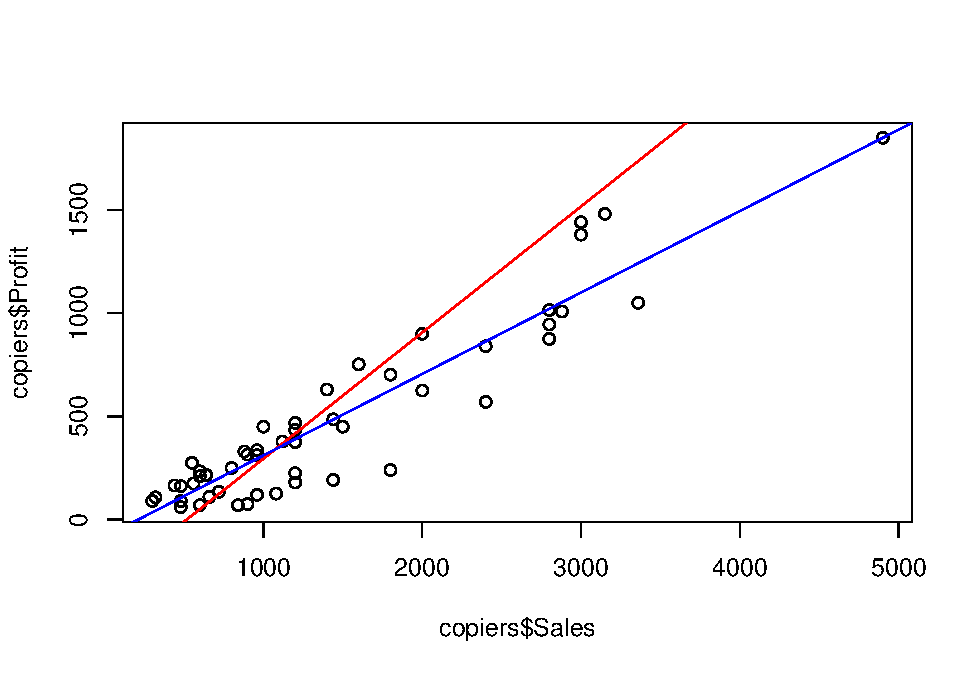
\includegraphics{PS_files/figure-latex/unnamed-chunk-24-1.pdf}

When a measurement follows a standard normal distribution, then the
assumptions of a normal distribution can be applied to the data and
these assumptions can be completely specified by two parameters, which
are the mean and standard deviation. The empirical rule of a standard
normal gives us the following:

\begin{itemize}
\tightlist
\item
  68\% of data will fall within 1 standard deviation of the mean\\
\item
  95\% of data will fall within 2 standard deviations of the mean
\item
  99.7\% of data will fall within 3 standard deviations of the mean
\end{itemize}

Scroll back to the normal curve we plotted above, observe:\\
- It is perfectly symmetrical - It is unimodal (has only a single
mode)\\
- Area under curve is 1

One relating idea that gives the normal distribution such significance
is known as the \textbf{Central limit theorem}: it says that when we
have many independent variables generated by all kinds of distributions,
the aggregate of those variables will tend toward a normal distribution
assuming of course the lack of any extraordinary intervention. This
universality is observed across different domains making the normal
distribution a core centerpiece in applied statistics and mathematics.

As an exercise, I'd like you to generate 50 random numbers using
\texttt{rnorm(50,\ 0,\ 1)} indicating mean of 0 and standard deviation
of 1. Print the result. Now, go ahead and save that as a variable, say,
\texttt{x}. You can use \texttt{density()} in conjunction with
\texttt{plot()} to now plot the 50 random numbers:

\begin{Shaded}
\begin{Highlighting}[]
\NormalTok{x =}\StringTok{ }\KeywordTok{rnorm}\NormalTok{(}\DecValTok{50}\NormalTok{,}\DecValTok{0}\NormalTok{,}\DecValTok{1}\NormalTok{)}
\KeywordTok{plot}\NormalTok{(}\KeywordTok{density}\NormalTok{(x))}
\end{Highlighting}
\end{Shaded}

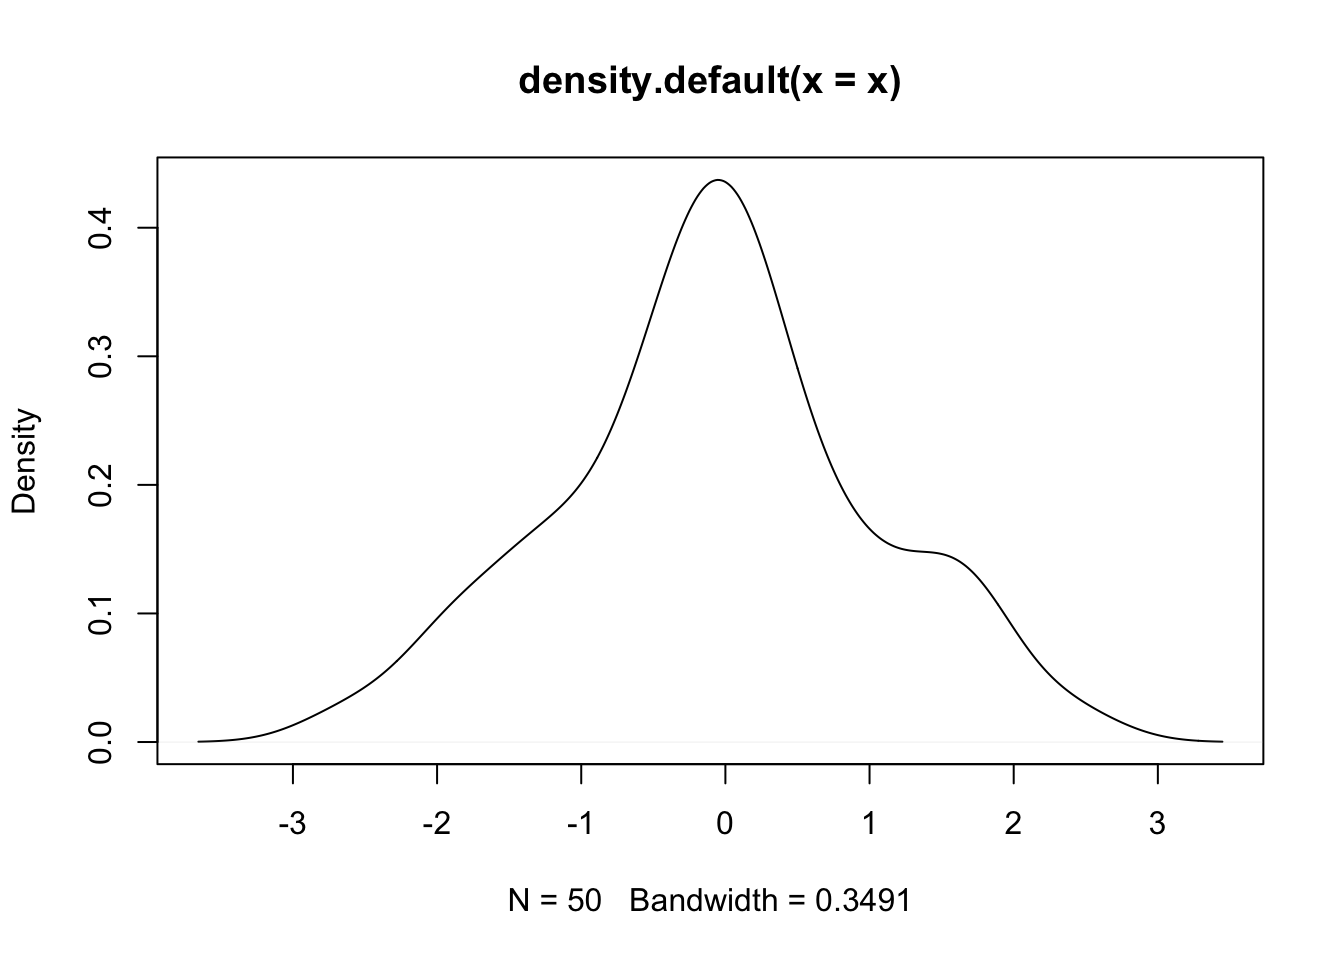
\includegraphics{PS_files/figure-latex/unnamed-chunk-25-1.pdf}

Supposed you were to change 50 to 500, and then to 5000 and even 50000,
what did you observe? The key takeaway here is that as the number of
sample approach infinity this plot will eventually converge in
distribution to the standard normal.

Take some time to work through the above concepts if any of these are
new to you. When you're ready, we're hop into inferential statistics and
talk about continuous random variables and the \textbf{probability
density function}.

\hypertarget{inferential-statistics}{%
\section{Inferential Statistics}\label{inferential-statistics}}

\hypertarget{probability-density-function}{%
\subsection{Probability Density
Function}\label{probability-density-function}}

When we're thinking about continuous random variables (blood sugar
level, height, rainfall amount), it is important to realize that this
variable has an uncountable number of possible values, even between two
real intervals. The resulting probability distribution of the variable
can be described by a probability density, where the probability is
found by taking the area under the curve.

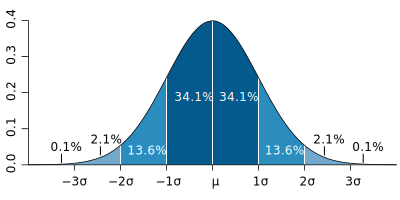
\includegraphics{assets/pdf.svg}

\hypertarget{probability-mass-function}{%
\subsection{Probability Mass Function}\label{probability-mass-function}}

Discrete random variables (number of player injury, amount of defaulted
loans, travel bookings per customer), on the other hand, can be
described using a probability mass function, which maps each value of
the random variable to a probability:\\
- p(0 bookings) = 0.28\\
- p(1 booking) = 0.09\\
\ldots{} - p(6 bookings) = 0.004

Because they are probabilities, these individual probabilities have to
sum up to 1.

\hypertarget{real-life-examples-why-these-attributes-are-important}{%
\subsection{Real Life Examples: Why these attributes are
important}\label{real-life-examples-why-these-attributes-are-important}}

Going back to the standard normal distribution - you may be asking by
now how any of what you're learning in the past few chapters are useful.
To answer the question, I feel it is only appropriate we solidify these
intuition with a few concrete examples. Consider the following scenario:

The height of men in Indonesia is normally distributed with a mean of
160cm and a standard deviation of 7cm. What is the probability of a
randomly selected man being taller than 175cm?

The solution: 175cm is 15cm above the mean, and dividing that by the
standard deviation of 7cm, we get 2.143. We refer to this as the
\emph{z-score}. The probability of an Indonesian men being taller than
175cm is P(Z \textgreater{} 2.143)

\begin{Shaded}
\begin{Highlighting}[]
\NormalTok{z <-}\StringTok{ }\NormalTok{(}\DecValTok{175-160}\NormalTok{)}\OperatorTok{/}\DecValTok{7}
\KeywordTok{pnorm}\NormalTok{(z, }\DataTypeTok{lower.tail=}\NormalTok{F)}
\end{Highlighting}
\end{Shaded}

\begin{verbatim}
## [1] 0.01606229
\end{verbatim}

\begin{Shaded}
\begin{Highlighting}[]
\CommentTok{# equivalent: 1-pnorm(z)}
\end{Highlighting}
\end{Shaded}

\textbf{Quiz 2: Supposed we have a population mean of 180cm and standard
deviation of 8cm, what is the probability that a randomly picked person
being shorter than 174cm?}

\begin{Shaded}
\begin{Highlighting}[]
\CommentTok{#====Your Solution====}
\end{Highlighting}
\end{Shaded}

The Z-scores we used above is useful when relating different measurement
distributions to each acting as a common denominator. Essentially, a
z-score gives us a ``standardized'' unit that measure how many standard
deviations is a particular statistic away from the mean. This property,
as we'll see, is paramount to many statistical hypothesis tests,
performance evaluation (more of that when we get to the Machine Learning
courses), and in the construction of confidence or prediction intervals.

\hypertarget{confidence-intervals}{%
\subsection{Confidence Intervals}\label{confidence-intervals}}

To summarize what we've learned so far: - Populations are characterized
by descriptive statistics (``parameters'')\\
- Inferences about these parameters are drawn from sample statistics\\
- In estimating the population parameters we want to quantify the
certainty or reliability of our estimates

We often begin our estimation with a point estimate, using for example
the sample mean \(\bar{x}\) as a point estimate of the population mean
\(\mu\). We can then construct confidence intervals around our point
estimates so we have an interval that may contain the true value of the
parameter. When statisticians say a ``95\% confidence interval'', what
they mean is that if we create 100 confidence intervals of the same size
from a given population, we expect to find the true parameter (let's say
the population's net savings per household) in 95 of them.

We construct a confidence interval by taking the point estimate +/-
margin of error, where margin of error is computed as:\\
\(E = Z_{\alpha/2} * \frac{\sigma}{\sqrt{n}}\)

Because confidence intervals are two-sided the level of significance we
chose (alpha) has to be divided into halves. When we compute by finding
the z-score associated with a value of 2.5\% (0.025) on each end, we end
up looking at the middle 95\% of the area under the curve. We can use
\texttt{qnorm(0.025)} to help us find the z-score associated with a 95\%
confidence interval.

\begin{Shaded}
\begin{Highlighting}[]
\CommentTok{# 95% confidence interval}
\KeywordTok{qnorm}\NormalTok{(}\FloatTok{0.025}\NormalTok{)}
\end{Highlighting}
\end{Shaded}

\begin{verbatim}
## [1] -1.959964
\end{verbatim}

\begin{Shaded}
\begin{Highlighting}[]
\CommentTok{# 99% confidence interval}
\KeywordTok{qnorm}\NormalTok{(}\FloatTok{0.005}\NormalTok{)}
\end{Highlighting}
\end{Shaded}

\begin{verbatim}
## [1] -2.575829
\end{verbatim}

Again, let's put together a scenario to make all of this more concrete.
Say we want to know the average annual dividend payout in a particular
industry, and had known through an earlier study that this figure
resembles a normal distribution with a population standard deviation of
2.4\%. We looked at the public books of these 81 companies in said
industry and attain a sample mean of 11.8\% (that is, the average
company from this group of 81 companies pay 11.8\% of profit to their
shareholders annually). We want to construct a 95\% confidence interval
for the \(\mu\), the mean dividend payout.

Solution: - Z-score associated with a 95\% confidence interval is 1.96\\
- The standard error of the mean (SE) is 2.4/sqrt(81) = 0.267 - The
margin of error (E) is 1.96*SE = 0.524\\
- The confidence interval is 11.8\% +- 0.524\%

And so we can say that the 95\% confidence interval for the mean
dividend payout in this industry is \textbf{(11.28\%, 12.32\%)}. We can
be 95\% confident that this interval will contain the mean dividend
payout for this particular industry.

\hypertarget{hypothesis-test-and-p-value}{%
\subsection{Hypothesis Test and
p-value}\label{hypothesis-test-and-p-value}}

In your day to day data science work, you will often be required to
explain the model's reliability and uncertainty, and the formal process
of such is specified as something called the \textbf{test of
significance}. Statistical significance often reference the
\textbf{p-value}, a measure of the probability of obtaining a result
equal to or more extreme than what was actually observed, assuming the
null hypothesis is true.

Imagine a scenario where you're assigned to consult on Quicker, a
startup that simplify and automate government grants application for
newly incorporated startups. Through public announcements and official
records, you find that the average duration for a newly incorporated
startup to get its first government grant or financial funding is 215
days (with a population standard variance of 24 days, again through
official records). Of the 35 entrepreneurs using Quicker platform, the
average time is 178 days.

\textbf{Quiz 3: Does this observation (178 days) deviate away from the
population enough for it to be statistically significant? Use a 95\%
confidence interval}

The null hypothesis is \(H_0: \mu = \mu_0\)\\
The alternative hypothesis is: \(H_A: \mu < \mu_0\)

The null hypothesis is that our new mean \textbf{equals to} the original
mean, whereas the alternative hypothesis states that the mean of Quicker
customers \textbf{is lower than} the original mean.

Recall what we've learned about the z-score, we can compute the p-value
as follow:

\begin{Shaded}
\begin{Highlighting}[]
\NormalTok{z <-}\StringTok{ }\NormalTok{(}\DecValTok{178-215}\NormalTok{)}\OperatorTok{/}\DecValTok{24}
\KeywordTok{pnorm}\NormalTok{(z)}
\end{Highlighting}
\end{Shaded}

\begin{verbatim}
## [1] 0.06157731
\end{verbatim}

\begin{Shaded}
\begin{Highlighting}[]
\CommentTok{# equivalent: pnorm(178, 215, 24)}
\end{Highlighting}
\end{Shaded}

While we can reject the null hypothesis at the 95\% confidence level if
our p-value is \textless{}= alpha (0.05), this is not the case here as
our p-value is actually 0.0616. In this scenario, we fail to reject the
null hypothesis that the Quicker platform did in fact led to a
statistically significant reduction in government funding time.

\hypertarget{t-test}{%
\subsection{T-Test}\label{t-test}}

Generally, z-tests are used when we have a large enough sample size
(rule of thumb is n \textgreater{}= 30) and when the population standard
deviation is known. If the above conditions aren't met, we can instead
use a statistical measurement known as the Student's t-test. Say grant
automation platform has 10 users so far, and below is a vector named
\texttt{duration} that stores the number of days it takes for their
first government funding. Supposed also that the population standard
deviation (sigma) is not known.

In R we can use \texttt{t.test(x,\ mu)} and pass in an optional
alternative hypothesis. Here we're interested in finding out whether we
can reject the null hypothesis (that says there is no difference in
government funding time for Quicker startups and other startups) in
favor of the alternative hypothesis (that Quicker startup spend
\textbf{less} time on average to acquire their first grant):

\begin{Shaded}
\begin{Highlighting}[]
\NormalTok{duration <-}\StringTok{ }\KeywordTok{c}\NormalTok{(}\DecValTok{184}\NormalTok{, }\DecValTok{181}\NormalTok{, }\DecValTok{230}\NormalTok{, }\DecValTok{169}\NormalTok{, }\DecValTok{158}\NormalTok{, }\DecValTok{204}\NormalTok{, }\DecValTok{220}\NormalTok{, }\DecValTok{197}\NormalTok{, }\DecValTok{219}\NormalTok{, }\DecValTok{223}\NormalTok{)}
\KeywordTok{t.test}\NormalTok{(duration, }\DataTypeTok{mu=}\DecValTok{215}\NormalTok{, }\DataTypeTok{alternative =} \StringTok{"less"}\NormalTok{)}
\end{Highlighting}
\end{Shaded}

\begin{verbatim}
## 
##  One Sample t-test
## 
## data:  duration
## t = -2.1041, df = 9, p-value = 0.03234
## alternative hypothesis: true mean is less than 215
## 95 percent confidence interval:
##     -Inf 212.875
## sample estimates:
## mean of x 
##     198.5
\end{verbatim}

As you progress along the Machine Learning Specialization, many of the
models you will come across will inevitably make use of these
statistical tools we have discussed. You will see plenty application of
p-values, confidence intervals, and the numerous statistical methods
we've just learned.

Because this is a \textbf{Practical Statistics} workshop, I want to
dedicate the following chapter to tips and techniques you can
incorporate into your data science work using the goodness that has been
baked into R.

\hypertarget{tips-and-techniques-working-with-statistics-in-r}{%
\section{Tips and Techniques: Working with Statistics in
R}\label{tips-and-techniques-working-with-statistics-in-r}}

\begin{enumerate}
\def\labelenumi{\arabic{enumi}.}
\tightlist
\item
  Density Plots
\end{enumerate}

\begin{Shaded}
\begin{Highlighting}[]
\KeywordTok{plot}\NormalTok{(}\KeywordTok{density}\NormalTok{(retail}\OperatorTok{$}\NormalTok{Profit, }\DataTypeTok{from=}\OperatorTok{-}\DecValTok{100}\NormalTok{, }\DataTypeTok{to=}\DecValTok{100}\NormalTok{))}
\end{Highlighting}
\end{Shaded}

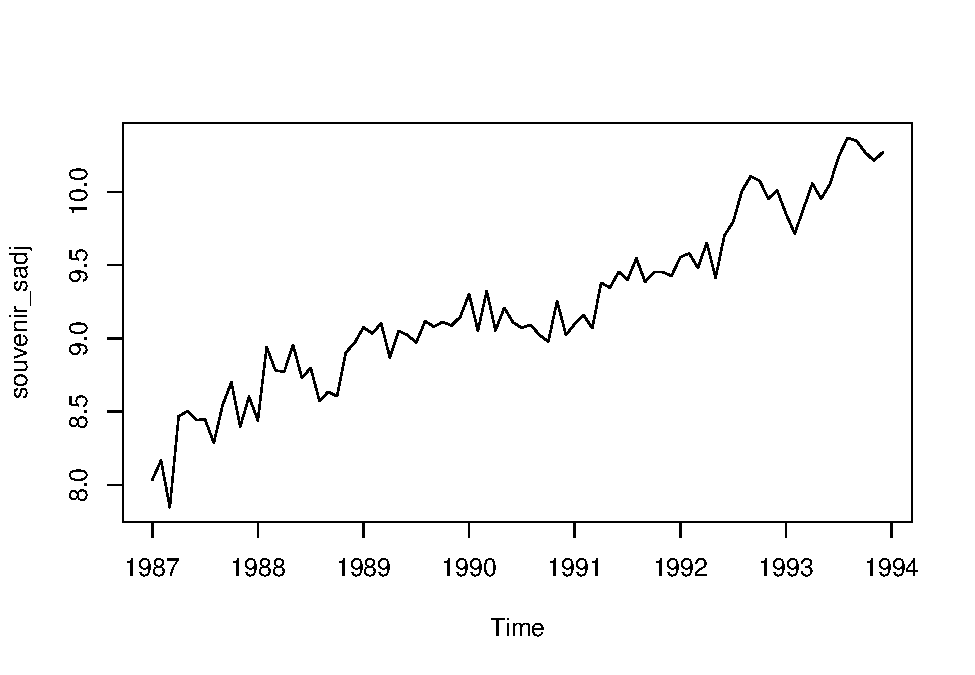
\includegraphics{PS_files/figure-latex/unnamed-chunk-31-1.pdf}

\begin{Shaded}
\begin{Highlighting}[]
\KeywordTok{plot}\NormalTok{(}\KeywordTok{density}\NormalTok{(retail}\OperatorTok{$}\NormalTok{Profit, }\DataTypeTok{from=}\OperatorTok{-}\DecValTok{100}\NormalTok{, }\DataTypeTok{to=}\DecValTok{100}\NormalTok{), }\DataTypeTok{col=}\StringTok{"goldenrod3"}\NormalTok{)}
\KeywordTok{lines}\NormalTok{(}\KeywordTok{density}\NormalTok{(retail}\OperatorTok{$}\NormalTok{Sales), }\DataTypeTok{col=}\StringTok{"dodgerblue2"}\NormalTok{)}
\end{Highlighting}
\end{Shaded}

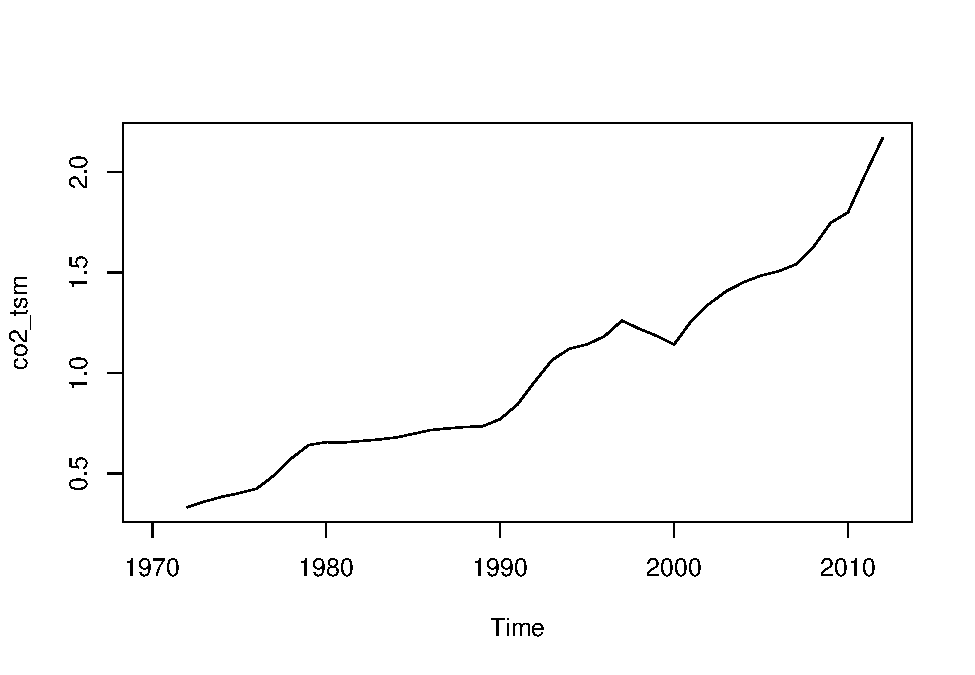
\includegraphics{PS_files/figure-latex/unnamed-chunk-32-1.pdf}

\begin{enumerate}
\def\labelenumi{\arabic{enumi}.}
\setcounter{enumi}{1}
\tightlist
\item
  Boxplots
\end{enumerate}

\begin{Shaded}
\begin{Highlighting}[]
\KeywordTok{boxplot}\NormalTok{(Profit }\OperatorTok{~}\StringTok{ }\NormalTok{Category, retail, }\DataTypeTok{ylim=}\KeywordTok{c}\NormalTok{(}\OperatorTok{-}\DecValTok{100}\NormalTok{, }\DecValTok{100}\NormalTok{))}
\end{Highlighting}
\end{Shaded}

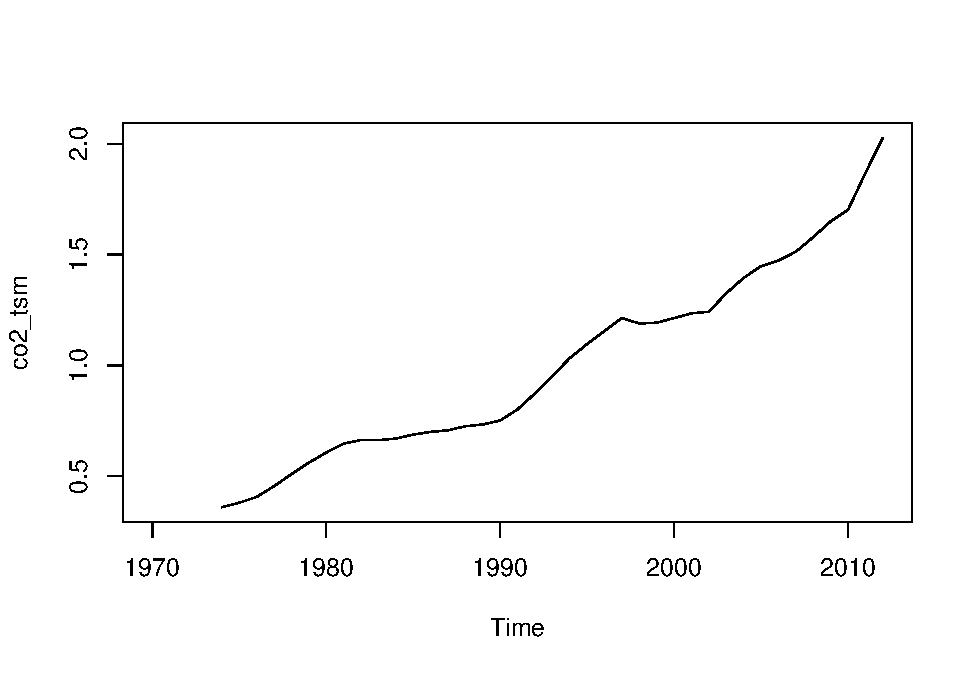
\includegraphics{PS_files/figure-latex/unnamed-chunk-33-1.pdf}

\begin{enumerate}
\def\labelenumi{\arabic{enumi}.}
\setcounter{enumi}{2}
\tightlist
\item
  Using \texttt{skim()} for better summary statistics:
\end{enumerate}

\begin{Shaded}
\begin{Highlighting}[]
\KeywordTok{library}\NormalTok{(skimr)}
\CommentTok{# skim(retail[,c("Sales", "Quantity", "Discount", "Profit")])}
\KeywordTok{skim}\NormalTok{(retail[,}\DecValTok{10}\OperatorTok{:}\DecValTok{13}\NormalTok{])}
\end{Highlighting}
\end{Shaded}

\begin{longtable}[]{@{}ll@{}}
\caption{Data summary}\tabularnewline
\toprule
\endhead
Name & retail{[}, 10:13{]}\tabularnewline
Number of rows & 9994\tabularnewline
Number of columns & 4\tabularnewline
\_\_\_\_\_\_\_\_\_\_\_\_\_\_\_\_\_\_\_\_\_\_\_ &\tabularnewline
Column type frequency: &\tabularnewline
numeric & 4\tabularnewline
\_\_\_\_\_\_\_\_\_\_\_\_\_\_\_\_\_\_\_\_\_\_\_\_ &\tabularnewline
Group variables & None\tabularnewline
\bottomrule
\end{longtable}

\textbf{Variable type: numeric}

\begin{longtable}[]{@{}lrrrrrrrrrl@{}}
\toprule
skim\_variable & n\_missing & complete\_rate & mean & sd & p0 & p25 &
p50 & p75 & p100 & hist\tabularnewline
\midrule
\endhead
Sales & 0 & 1 & 229.86 & 623.25 & 0.44 & 17.28 & 54.49 & 209.94 &
22638.48 & ▇▁▁▁▁\tabularnewline
Quantity & 0 & 1 & 3.79 & 2.23 & 1.00 & 2.00 & 3.00 & 5.00 & 14.00 &
▇▅▁▁▁\tabularnewline
Discount & 0 & 1 & 0.16 & 0.21 & 0.00 & 0.00 & 0.20 & 0.20 & 0.80 &
▇▆▁▁▁\tabularnewline
Profit & 0 & 1 & 28.66 & 234.26 & -6599.98 & 1.73 & 8.67 & 29.36 &
8399.98 & ▁▁▇▁▁\tabularnewline
\bottomrule
\end{longtable}

\begin{enumerate}
\def\labelenumi{\arabic{enumi}.}
\setcounter{enumi}{3}
\tightlist
\item
  Pairs Matrix
\end{enumerate}

\begin{Shaded}
\begin{Highlighting}[]
\KeywordTok{pairs}\NormalTok{(retail[,}\KeywordTok{c}\NormalTok{(}\StringTok{"Sales"}\NormalTok{, }\StringTok{"Quantity"}\NormalTok{, }\StringTok{"Discount"}\NormalTok{, }\StringTok{"Profit"}\NormalTok{)])}
\end{Highlighting}
\end{Shaded}

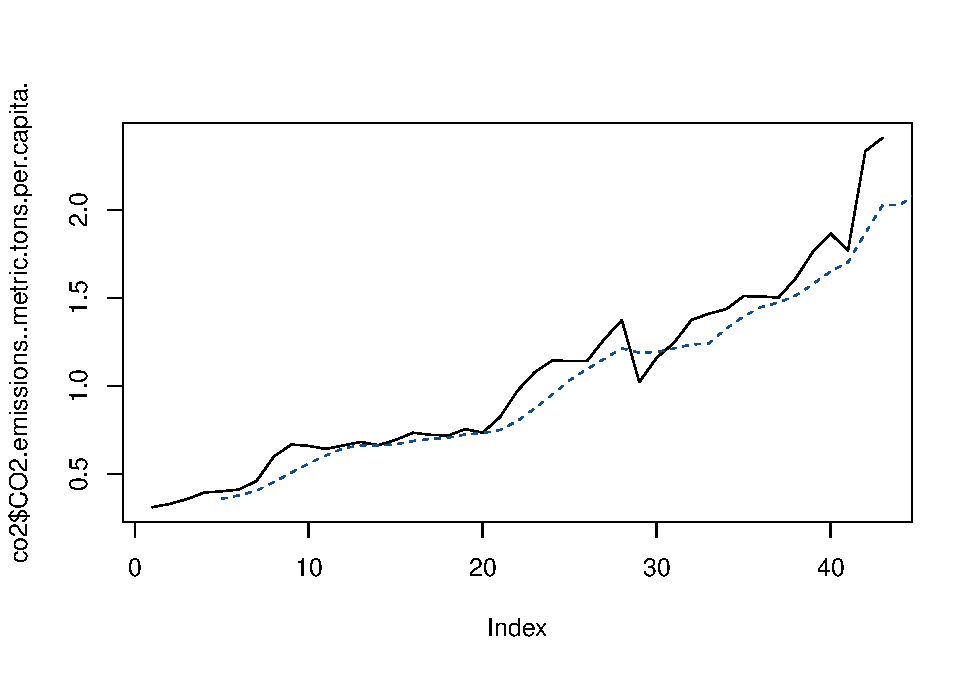
\includegraphics{PS_files/figure-latex/unnamed-chunk-35-1.pdf}

\begin{Shaded}
\begin{Highlighting}[]
\CommentTok{# 2x2 pictures on one plot, square plotting region}
\NormalTok{op <-}\StringTok{ }\KeywordTok{par}\NormalTok{(}\DataTypeTok{mfrow=}\KeywordTok{c}\NormalTok{(}\DecValTok{2}\NormalTok{,}\DecValTok{2}\NormalTok{), }\DataTypeTok{pty=}\StringTok{"s"}\NormalTok{)}

\KeywordTok{par}\NormalTok{(}\DataTypeTok{mfrow=}\KeywordTok{c}\NormalTok{(}\DecValTok{1}\NormalTok{,}\DecValTok{3}\NormalTok{))}
\KeywordTok{hist}\NormalTok{(retail}\OperatorTok{$}\NormalTok{Sales, }\DataTypeTok{breaks =} \DecValTok{100}\NormalTok{, }\DataTypeTok{xlim=}\KeywordTok{c}\NormalTok{(}\DecValTok{0}\NormalTok{,}\DecValTok{2500}\NormalTok{), }\DataTypeTok{main=}\StringTok{""}\NormalTok{)}
\KeywordTok{plot}\NormalTok{(}\KeywordTok{density}\NormalTok{(retail}\OperatorTok{$}\NormalTok{Sales, }\DataTypeTok{from=}\DecValTok{0}\NormalTok{, }\DataTypeTok{to=}\DecValTok{2500}\NormalTok{), }\DataTypeTok{main=}\StringTok{""}\NormalTok{)}
\KeywordTok{plot}\NormalTok{(}\KeywordTok{sort}\NormalTok{(retail}\OperatorTok{$}\NormalTok{Sales), }\DataTypeTok{pch=}\StringTok{"."}\NormalTok{)}
\KeywordTok{title}\NormalTok{(}\DataTypeTok{main =} \StringTok{"Three Statistical Plots"}\NormalTok{, }\DataTypeTok{outer =}\NormalTok{ T)}
\end{Highlighting}
\end{Shaded}

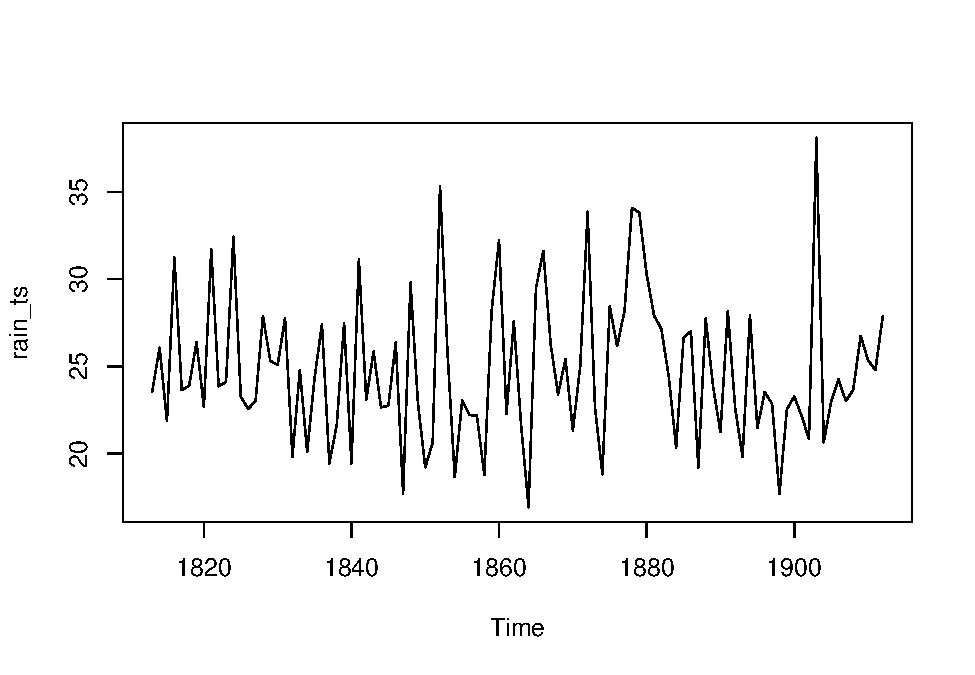
\includegraphics{PS_files/figure-latex/unnamed-chunk-36-1.pdf}

\begin{Shaded}
\begin{Highlighting}[]
\CommentTok{# end of plotting, reset to previous settings}
\KeywordTok{par}\NormalTok{(op)}
\end{Highlighting}
\end{Shaded}

\textbf{Learn-By-Building: Statistical Treatment of Retail Dataset}\\
Using what you've learned, formulate a question and derive a statistical
hypothesis test to answer the question. You have to demonstrate that
you're able to make decisions using data in a scientific manner.
Examples of questions can be:\\
- Is there a different in profitability between standard shipment and
same-day shipment?\\
- Supposed there is no difference in profitability between the different
product segment, what is the probability that we obtain the current
observation due to pure chance alone?

You can think about the kind of business question you'd like to tackle,
and you are free to choose the reasonable parameters for your confidence
intervals and other statistical tests. Explain your decision-making
process.

This learn-by-building module is not graded.

\hypertarget{additional-remarks}{%
\section{Additional Remarks}\label{additional-remarks}}

\end{document}
